
%% ----------------------------------------------------------------
%% Article.tex
%% ----------------------------------------------------------------
% Koma-script replacement article document class
\documentclass{ecsreport}

% List customisation package
\usepackage{enumitem}
\usepackage[refpage]{nomencl}

% Format hyphenations with britain specific formatting
\usepackage[british]{babel}
% Bibliographic citation engine
\usepackage{natbib}            % Use Natbib style for the refs.
% Package for correct handeling of urls, email addresses etc...
\usepackage{url}
% Allows for manual handeling of object and figure placement
\usepackage{float}
% Handles captioning of objects and figures
\usepackage{caption}
% Place captions on top of table
\restylefloat{table}

\usepackage[table]{xcolor}
\usepackage{booktabs}
\usepackage{tabulary}
\usepackage[pass]{geometry}
\usepackage{pdflscape}
\usepackage{graphicx}

% Gantt chart
\usepackage{pgfgantt}
\usepackage{tikz}
\usepackage{varwidth}
\usepackage{ragged2e}
\newganttlinktype{rdldr*}{%
  \draw [/pgfgantt/link]
    (\xLeft, \yUpper) --
    (\xLeft + \ganttvalueof{link bulge 1} * \ganttvalueof{x unit},
      \yUpper) --
    ($(\xLeft + \ganttvalueof{link bulge 1} * \ganttvalueof{x unit},
      \yUpper)!%
      \ganttvalueof{link mid}!%
      (\xLeft + \ganttvalueof{link bulge 1} * \ganttvalueof{x unit},
      \yLower)$) --
    ($(\xRight - \ganttvalueof{link bulge 2} * \ganttvalueof{x unit},
      \yUpper)!%
      \ganttvalueof{link mid}!%
      (\xRight - \ganttvalueof{link bulge 2} * \ganttvalueof{x unit},
      \yLower)$) --
    (\xRight - \ganttvalueof{link bulge 2} * \ganttvalueof{x unit},
      \yLower) --
    (\xRight, \yLower);%
}
\ganttset{
  link bulge 1/.link=/pgfgantt/link bulge,
  link bulge 2/.link=/pgfgantt/link bulge}

\usetikzlibrary{arrows,positioning,shapes.geometric}

\newcommand{\dtoprule}{\specialrule{1pt}{0pt}{1.4pt}%
            \specialrule{1pt}{0pt}{0pt}%
            }
\newcommand{\dbottomrule}{\specialrule{1pt}{0pt}{1.4pt}%
            \specialrule{1pt}{0pt}{\belowrulesep}%
            }
\newcommand{\emidrule}{\specialrule{0.5pt}{0pt}{1.4pt}%
            }
% Allow counters for footers to be reset per page
\usepackage{perpage}
\MakePerPage{footnote}
% Allows for manual control of abstract environment
\usepackage{abstract}
% Allow for inserting of images
\usepackage{graphicx}
% Create hyperlinks in bibliography
\usepackage{hyperref}
% Enhanced mathemeatical formating
\usepackage{amsmath}
% Included for issues to do with fonts and accents. Nothing worth worrying
% about...
\usepackage[T1]{fontenc}
% Write in utf-8. Just leave it and don't worry about it...
\usepackage[utf8]{inputenc}
% Used for adding lorum ipsum filler text
\usepackage{blindtext}
% Set path to included figures and graphics
\graphicspath{./resources/}

\usepackage{tipa}
% Set path to bibliography location
% 
% Post-process bibliography for special characters - a workaround for a
% problem with Mendley's handling of certain characters in hyperlinks
% \DeclareSourcemap{
%     \maps{
%         \map{ % Replaces '{\_}', '{_}' or '\_' with just '_'
%             \step[fieldsource=url,
%                   match=\regexp{\{\\\_\}|\{\_\}|\\\_},
%                   replace=\regexp{\_}]
%         }
%         \map{ % Replaces '{'$\sim$'}', '$\sim$' or '{~}' with just '~'
%             \step[fieldsource=url,
%                   match=\regexp{\{\$\\sim\$\}|\{\~\}|\$\\sim\$},
%                   replace=\regexp{\~}]
%         }
%     }
% }
% 
% % Place abstract on title page rather than on it's own separate page
% \newsavebox{\abstractbox}
% \renewenvironment{abstract}
%   {\begin{lrbox}{0}\begin{minipage}{\textwidth}
%    \begin{center}\normalfont\sectfont\abstractname\end{center}\quotation}
%   {\endquotation\end{minipage}\end{lrbox}%
%    \global\setbox\abstractbox=\box0 }
% 
% % No idea what this does...
% \usepackage{etoolbox}
% \makeatletter
% \expandafter\patchcmd\csname\string\maketitle\endcsname
%   {\vskip\z@\@plus3fill}
%   {\vskip\z@\@plus2fill\box\abstractbox\vskip\z@\@plus1fill}
%   {}{}
% \makeatother
% 
% % Declare \citeyearpar command for adding year (with paraentheses) without
% % author's name as reference
% \DeclareCiteCommand{\citeyearpar}
%     {}
%     {\mkbibparens{\bibhyperref{\printdate}}}
%     {\multicitedelim}
%     {}
% 
% MATLAB Code block stuff...
\usepackage{color}
\usepackage{listings}

\definecolor{dkgreen}{rgb}{0,0.6,0}
\definecolor{gray}{rgb}{0.5,0.5,0.5}
\definecolor{codegreen}{rgb}{0,0.6,0}
\definecolor{codegray}{rgb}{0.5,0.5,0.5}
\definecolor{codepurple}{rgb}{0.58,0,0.82}
\definecolor{backcolour}{rgb}{0.95,0.95,0.92}

\lstset{language=Matlab,
   keywords={break,case,catch,continue,else,elseif,end,for,function,
      global,if,otherwise,persistent,return,switch,try,while},
   basicstyle=\ttfamily,
   keywordstyle=\color{blue},
   commentstyle=\color{gray},
   stringstyle=\color{dkgreen},
   numbers=left,
   numberstyle=\tiny\color{gray},
   stepnumber=1,
   numbersep=10pt,
   backgroundcolor=\color{white},
   tabsize=4,
   showspaces=false,
   showstringspaces=false}
            % Include your abbreviations
\graphicspath{{./resources/}}
\hypersetup{colorlinks=true}   % Set to false for black/white printing
\input{Definitions}            % Include your abbreviations
%% ----------------------------------------------------------------
\begin{document}

\frontmatter
\title      {Speech in noise test battery development plan}
\authors    {\texorpdfstring
             {\href{mailto:s.w.perry@soton.ac.uk}{Samuel W. Perry}}
             {Samuel W. Perry}
            }
\addresses  {\groupname\\\deptname\\\univname}
\date       {\today}
\subject    {}
\keywords   {}
\maketitle
\mainmatter
%% ----------------------------------------------------------------
\section*{Outline}\label{Section:Introduction}
\begin{itemize}
    \item Initial task is to develop a speech in noise test such as BKB in a
        portable format that could be deployed on a standard Windows (or Mac)
        based system easily, thus improving on the original Matlab implementation.
    \item Results of test presented on screen to clinician in initial
        implementation, no further management of data.
    \item Further development then focused on management of patient data using
        Southampton's database. This is currently the most significant unknown
        in the project due to lack of details on database format and lack of
        prior experience with databases, relative to other skills.
    \item Other data export options may or may not be possible (such as
        exporting to an excel file). This will be determined through parallel
        work on the EHS project.
    \item Subsequent tests will then be implemented based on priority, liasing
        with clinicians to determine the details of any other features that may
        be of use.
    \item An estimated final delivery of early 2020 is proposed, however this
        is highly dependent on unknown factors such as the database and the
        number of speech in noise tests to be developed.  Additionally, as this
        project is running in parallel with both the developer's PhD work and
        the EHS project, other projects may need to be prioritised at times
        based on their progress.
\end{itemize}

\begin{landscape}
\section*{Project timeline 1--10 months}\label{Section:Gantt}
\begin{figure}[H]
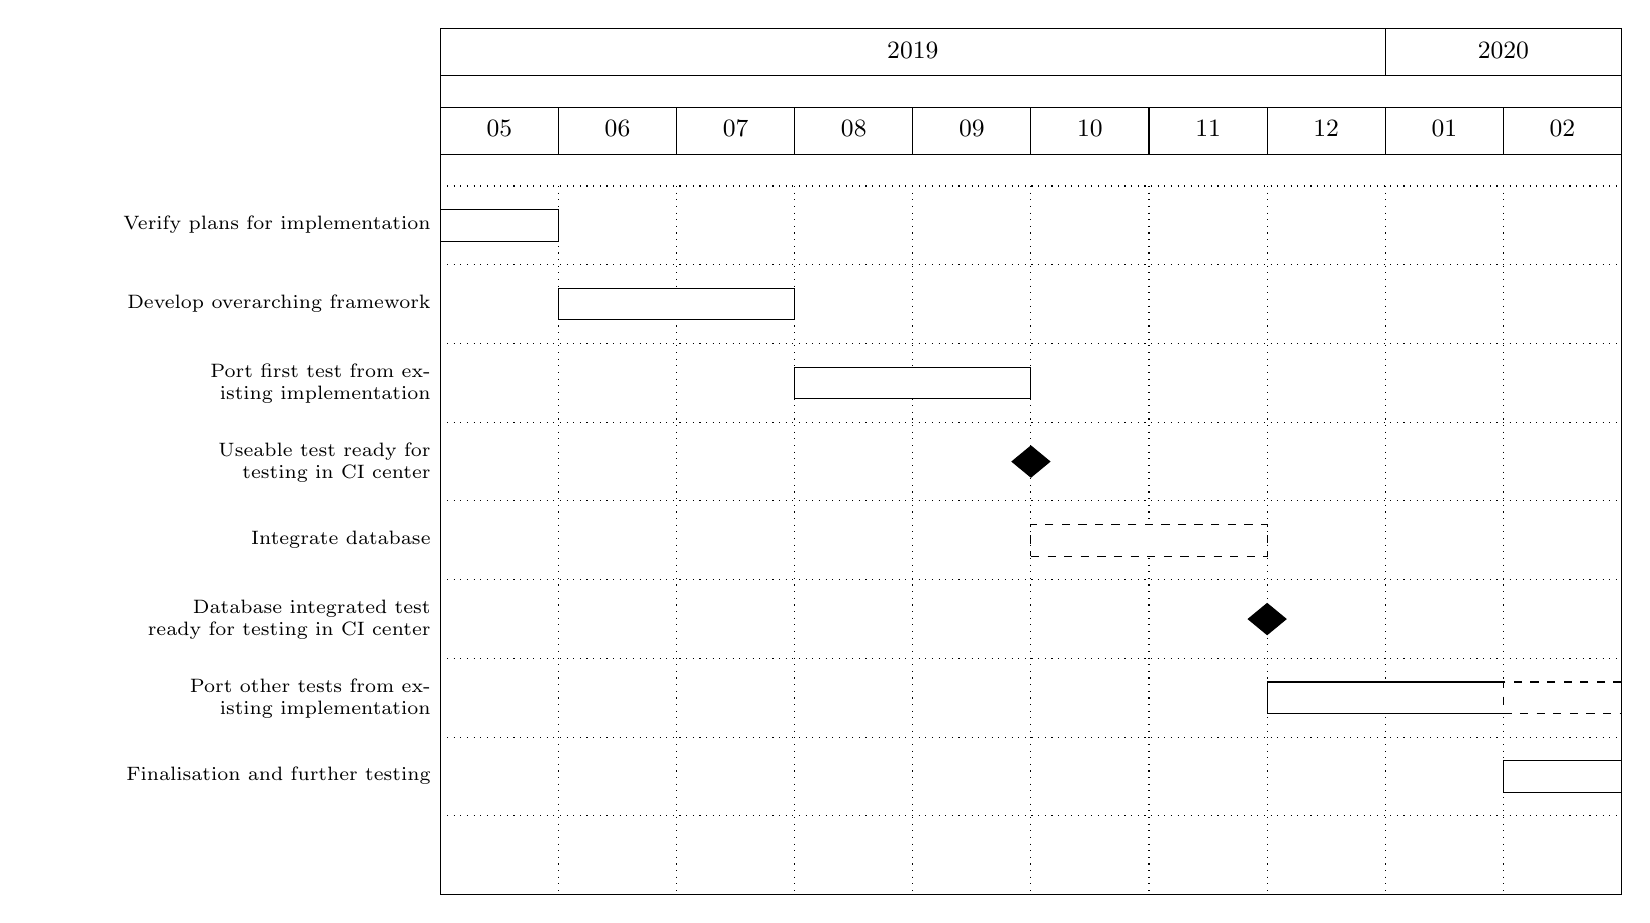
\begin{tikzpicture}
\begin{ganttchart}[
hgrid,
vgrid,
time slot format=isodate-yearmonth,
%progress label text=  {\quad\pgfmathprintnumber[precision=0,verbatim]{#1}\%},
milestone label font=\tiny,
%group label font=\tiny,
%title label font=\tiny,
bar label node/.style={text width=5cm,align=right,font=\scriptsize\RaggedLeft,anchor=east},
milestone label node/.style={text width=5cm,align=right,font=\scriptsize\RaggedLeft,anchor=east},
%group label node/.style={text width=3cm,align=right,font=\scriptsize\RaggedLeft,anchor=east}
time slot unit=month,
x unit=1.5cm,
milestone/.append style={xscale=0.4} % 0.6/1.4 ≈ 0.42857
]{2019-05}{2020-02}
\gantttitlecalendar{year, month} \\
% \ganttbar[bar/.append style={dashed}]{}{2019-02}{2019-09}
\ganttbar{Verify plans for implementation}{2019-05}{2019-05}\\
\ganttbar{Develop overarching framework}{2019-06}{2019-07}\\
\ganttbar{Port first test from existing implementation}{2019-08}{2019-09}\\
\ganttmilestone{Useable test ready for testing in CI center}{2019-09}\\
\ganttbar[bar/.append style={dashed}]{Integrate database}{2019-10}{2019-11}\\
\ganttmilestone{Database integrated test ready for testing in CI center}{2019-11}\\
\ganttbar{Port other tests from existing implementation}{2019-12}{2020-01}
\ganttbar[bar/.append style={dashed}]{}{2020-02}{2020-02}\\
\ganttbar{Finalisation and further testing}{2020-02}{2020-02}\\
\end{ganttchart}
\end{tikzpicture}
\caption*{Block tasks are unlikely to change in terms of timescales; dashed tasks may change due to technical challenges that are currently unknown; diamonds represent milestones}
\label{gantt}
\end{figure}
\end{landscape}
\end{document}
% ----------------------------------------------------------------
